% Created by tikzDevice version 0.12.6 on 2026-02-13 11:51:38
% !TEX encoding = UTF-8 Unicode
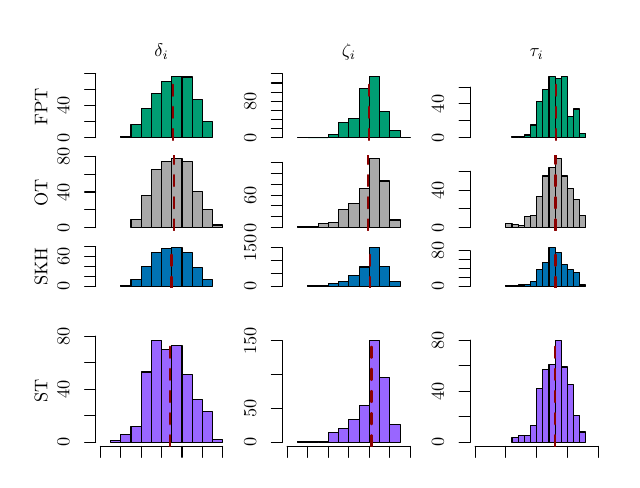
\begin{tikzpicture}[x=1pt,y=1pt]
\definecolor{fillColor}{RGB}{255,255,255}
\path[use as bounding box,fill=fillColor,fill opacity=0.00] (0,0) rectangle (211.10,156.03);
\begin{scope}
\path[clip] ( 24.55,115.43) rectangle ( 72.23,139.40);
\definecolor{drawColor}{RGB}{0,0,0}
\definecolor{fillColor}{RGB}{0,158,115}

\path[draw=drawColor,line width= 0.4pt,line join=round,line cap=round,fill=fillColor] ( 33.67,116.31) rectangle ( 37.35,116.60);

\path[draw=drawColor,line width= 0.4pt,line join=round,line cap=round,fill=fillColor] ( 37.35,116.31) rectangle ( 41.03,120.93);

\path[draw=drawColor,line width= 0.4pt,line join=round,line cap=round,fill=fillColor] ( 41.03,116.31) rectangle ( 44.71,126.98);

\path[draw=drawColor,line width= 0.4pt,line join=round,line cap=round,fill=fillColor] ( 44.71,116.31) rectangle ( 48.39,132.17);

\path[draw=drawColor,line width= 0.4pt,line join=round,line cap=round,fill=fillColor] ( 48.39,116.31) rectangle ( 52.07,136.49);

\path[draw=drawColor,line width= 0.4pt,line join=round,line cap=round,fill=fillColor] ( 52.07,116.31) rectangle ( 55.75,138.51);

\path[draw=drawColor,line width= 0.4pt,line join=round,line cap=round,fill=fillColor] ( 55.75,116.31) rectangle ( 59.42,138.22);

\path[draw=drawColor,line width= 0.4pt,line join=round,line cap=round,fill=fillColor] ( 59.42,116.31) rectangle ( 63.10,130.15);

\path[draw=drawColor,line width= 0.4pt,line join=round,line cap=round,fill=fillColor] ( 63.10,116.31) rectangle ( 66.78,122.08);
\end{scope}
\begin{scope}
\path[clip] (  0.00,  0.00) rectangle (211.10,156.03);
\definecolor{drawColor}{RGB}{0,0,0}

\path[draw=drawColor,line width= 0.4pt,line join=round,line cap=round] ( 24.55,116.31) -- ( 24.55,139.38);

\path[draw=drawColor,line width= 0.4pt,line join=round,line cap=round] ( 24.55,116.31) -- ( 20.59,116.31);

\path[draw=drawColor,line width= 0.4pt,line join=round,line cap=round] ( 24.55,122.08) -- ( 20.59,122.08);

\path[draw=drawColor,line width= 0.4pt,line join=round,line cap=round] ( 24.55,127.84) -- ( 20.59,127.84);

\path[draw=drawColor,line width= 0.4pt,line join=round,line cap=round] ( 24.55,133.61) -- ( 20.59,133.61);

\path[draw=drawColor,line width= 0.4pt,line join=round,line cap=round] ( 24.55,139.38) -- ( 20.59,139.38);

\node[text=drawColor,rotate= 90.00,anchor=base,inner sep=0pt, outer sep=0pt, scale=  0.66] at ( 15.05,116.31) {0};

\node[text=drawColor,rotate= 90.00,anchor=base,inner sep=0pt, outer sep=0pt, scale=  0.66] at ( 15.05,127.84) {40};
\end{scope}
\begin{scope}
\path[clip] (  0.00,110.67) rectangle ( 75.39,156.03);
\definecolor{drawColor}{RGB}{0,0,0}

\node[text=drawColor,anchor=base,inner sep=0pt, outer sep=0pt, scale=  0.66] at ( 48.39,145.44) {\bfseries $\delta_i$};

\node[text=drawColor,rotate= 90.00,anchor=base,inner sep=0pt, outer sep=0pt, scale=  0.66] at (  7.13,127.41) {FPT};
\end{scope}
\begin{scope}
\path[clip] ( 24.55,115.43) rectangle ( 72.23,139.40);
\definecolor{drawColor}{RGB}{139,0,0}

\path[draw=drawColor,line width= 0.8pt,dash pattern=on 4pt off 4pt ,line join=round,line cap=round] ( 52.64,115.43) -- ( 52.64,139.40);
\end{scope}
\begin{scope}
\path[clip] ( 92.03,115.43) rectangle (140.08,139.40);
\definecolor{drawColor}{RGB}{0,0,0}
\definecolor{fillColor}{RGB}{0,158,115}

\path[draw=drawColor,line width= 0.4pt,line join=round,line cap=round,fill=fillColor] ( 97.51,116.31) rectangle (101.22,116.48);

\path[draw=drawColor,line width= 0.4pt,line join=round,line cap=round,fill=fillColor] (101.22,116.31) rectangle (104.93,116.31);

\path[draw=drawColor,line width= 0.4pt,line join=round,line cap=round,fill=fillColor] (104.93,116.31) rectangle (108.64,116.31);

\path[draw=drawColor,line width= 0.4pt,line join=round,line cap=round,fill=fillColor] (108.64,116.31) rectangle (112.34,117.46);

\path[draw=drawColor,line width= 0.4pt,line join=round,line cap=round,fill=fillColor] (112.34,116.31) rectangle (116.05,121.74);

\path[draw=drawColor,line width= 0.4pt,line join=round,line cap=round,fill=fillColor] (116.05,116.31) rectangle (119.76,123.05);

\path[draw=drawColor,line width= 0.4pt,line join=round,line cap=round,fill=fillColor] (119.76,116.31) rectangle (123.47,134.07);

\path[draw=drawColor,line width= 0.4pt,line join=round,line cap=round,fill=fillColor] (123.47,116.31) rectangle (127.18,138.51);

\path[draw=drawColor,line width= 0.4pt,line join=round,line cap=round,fill=fillColor] (127.18,116.31) rectangle (130.88,125.85);

\path[draw=drawColor,line width= 0.4pt,line join=round,line cap=round,fill=fillColor] (130.88,116.31) rectangle (134.59,118.94);

\path[draw=drawColor,line width= 0.4pt,line join=round,line cap=round,fill=fillColor] (134.59,116.31) rectangle (138.30,116.48);
\end{scope}
\begin{scope}
\path[clip] (  0.00,  0.00) rectangle (211.10,156.03);
\definecolor{drawColor}{RGB}{0,0,0}

\path[draw=drawColor,line width= 0.4pt,line join=round,line cap=round] ( 92.03,116.31) -- ( 92.03,139.33);

\path[draw=drawColor,line width= 0.4pt,line join=round,line cap=round] ( 92.03,116.31) -- ( 88.07,116.31);

\path[draw=drawColor,line width= 0.4pt,line join=round,line cap=round] ( 92.03,119.60) -- ( 88.07,119.60);

\path[draw=drawColor,line width= 0.4pt,line join=round,line cap=round] ( 92.03,122.89) -- ( 88.07,122.89);

\path[draw=drawColor,line width= 0.4pt,line join=round,line cap=round] ( 92.03,126.18) -- ( 88.07,126.18);

\path[draw=drawColor,line width= 0.4pt,line join=round,line cap=round] ( 92.03,129.47) -- ( 88.07,129.47);

\path[draw=drawColor,line width= 0.4pt,line join=round,line cap=round] ( 92.03,132.76) -- ( 88.07,132.76);

\path[draw=drawColor,line width= 0.4pt,line join=round,line cap=round] ( 92.03,136.04) -- ( 88.07,136.04);

\path[draw=drawColor,line width= 0.4pt,line join=round,line cap=round] ( 92.03,139.33) -- ( 88.07,139.33);

\node[text=drawColor,rotate= 90.00,anchor=base,inner sep=0pt, outer sep=0pt, scale=  0.66] at ( 82.52,116.31) {0};

\node[text=drawColor,rotate= 90.00,anchor=base,inner sep=0pt, outer sep=0pt, scale=  0.66] at ( 82.52,129.47) {80};
\end{scope}
\begin{scope}
\path[clip] ( 75.39,110.67) rectangle (143.25,156.03);
\definecolor{drawColor}{RGB}{0,0,0}

\node[text=drawColor,anchor=base,inner sep=0pt, outer sep=0pt, scale=  0.66] at (116.05,145.44) {\bfseries $\zeta_i$};
\end{scope}
\begin{scope}
\path[clip] ( 92.03,115.43) rectangle (140.08,139.40);
\definecolor{drawColor}{RGB}{139,0,0}

\path[draw=drawColor,line width= 0.8pt,dash pattern=on 4pt off 4pt ,line join=round,line cap=round] (123.26,115.43) -- (123.26,139.40);
\end{scope}
\begin{scope}
\path[clip] (159.88,115.43) rectangle (207.93,139.40);
\definecolor{drawColor}{RGB}{0,0,0}
\definecolor{fillColor}{RGB}{0,158,115}

\path[draw=drawColor,line width= 0.4pt,line join=round,line cap=round,fill=fillColor] (175.01,116.31) rectangle (177.23,116.62);

\path[draw=drawColor,line width= 0.4pt,line join=round,line cap=round,fill=fillColor] (177.23,116.31) rectangle (179.46,116.62);

\path[draw=drawColor,line width= 0.4pt,line join=round,line cap=round,fill=fillColor] (179.46,116.31) rectangle (181.68,117.23);

\path[draw=drawColor,line width= 0.4pt,line join=round,line cap=round,fill=fillColor] (181.68,116.31) rectangle (183.91,120.87);

\path[draw=drawColor,line width= 0.4pt,line join=round,line cap=round,fill=fillColor] (183.91,116.31) rectangle (186.13,129.39);

\path[draw=drawColor,line width= 0.4pt,line join=round,line cap=round,fill=fillColor] (186.13,116.31) rectangle (188.36,133.65);

\path[draw=drawColor,line width= 0.4pt,line join=round,line cap=round,fill=fillColor] (188.36,116.31) rectangle (190.58,138.51);

\path[draw=drawColor,line width= 0.4pt,line join=round,line cap=round,fill=fillColor] (190.58,116.31) rectangle (192.80,137.60);

\path[draw=drawColor,line width= 0.4pt,line join=round,line cap=round,fill=fillColor] (192.80,116.31) rectangle (195.03,138.51);

\path[draw=drawColor,line width= 0.4pt,line join=round,line cap=round,fill=fillColor] (195.03,116.31) rectangle (197.25,123.92);

\path[draw=drawColor,line width= 0.4pt,line join=round,line cap=round,fill=fillColor] (197.25,116.31) rectangle (199.48,126.65);

\path[draw=drawColor,line width= 0.4pt,line join=round,line cap=round,fill=fillColor] (199.48,116.31) rectangle (201.70,117.83);
\end{scope}
\begin{scope}
\path[clip] (  0.00,  0.00) rectangle (211.10,156.03);
\definecolor{drawColor}{RGB}{0,0,0}

\path[draw=drawColor,line width= 0.4pt,line join=round,line cap=round] (159.88,116.31) -- (159.88,134.56);

\path[draw=drawColor,line width= 0.4pt,line join=round,line cap=round] (159.88,116.31) -- (155.92,116.31);

\path[draw=drawColor,line width= 0.4pt,line join=round,line cap=round] (159.88,122.39) -- (155.92,122.39);

\path[draw=drawColor,line width= 0.4pt,line join=round,line cap=round] (159.88,128.48) -- (155.92,128.48);

\path[draw=drawColor,line width= 0.4pt,line join=round,line cap=round] (159.88,134.56) -- (155.92,134.56);

\node[text=drawColor,rotate= 90.00,anchor=base,inner sep=0pt, outer sep=0pt, scale=  0.66] at (150.37,116.31) {0};

\node[text=drawColor,rotate= 90.00,anchor=base,inner sep=0pt, outer sep=0pt, scale=  0.66] at (150.37,128.48) {40};
\end{scope}
\begin{scope}
\path[clip] (143.25,110.67) rectangle (211.10,156.03);
\definecolor{drawColor}{RGB}{0,0,0}

\node[text=drawColor,anchor=base,inner sep=0pt, outer sep=0pt, scale=  0.66] at (183.91,145.44) {\bfseries $\tau_i$};
\end{scope}
\begin{scope}
\path[clip] (159.88,115.43) rectangle (207.93,139.40);
\definecolor{drawColor}{RGB}{139,0,0}

\path[draw=drawColor,line width= 0.8pt,dash pattern=on 4pt off 4pt ,line join=round,line cap=round] (190.80,115.43) -- (190.80,139.40);
\end{scope}
\begin{scope}
\path[clip] ( 24.55, 82.77) rectangle ( 72.23,109.88);
\definecolor{drawColor}{RGB}{0,0,0}
\definecolor{fillColor}{RGB}{169,169,169}

\path[draw=drawColor,line width= 0.4pt,line join=round,line cap=round,fill=fillColor] ( 37.35, 83.77) rectangle ( 41.03, 86.67);

\path[draw=drawColor,line width= 0.4pt,line join=round,line cap=round,fill=fillColor] ( 41.03, 83.77) rectangle ( 44.71, 95.36);

\path[draw=drawColor,line width= 0.4pt,line join=round,line cap=round,fill=fillColor] ( 44.71, 83.77) rectangle ( 48.39,104.69);

\path[draw=drawColor,line width= 0.4pt,line join=round,line cap=round,fill=fillColor] ( 48.39, 83.77) rectangle ( 52.07,107.59);

\path[draw=drawColor,line width= 0.4pt,line join=round,line cap=round,fill=fillColor] ( 52.07, 83.77) rectangle ( 55.75,108.88);

\path[draw=drawColor,line width= 0.4pt,line join=round,line cap=round,fill=fillColor] ( 55.75, 83.77) rectangle ( 59.42,107.59);

\path[draw=drawColor,line width= 0.4pt,line join=round,line cap=round,fill=fillColor] ( 59.42, 83.77) rectangle ( 63.10, 96.97);

\path[draw=drawColor,line width= 0.4pt,line join=round,line cap=round,fill=fillColor] ( 63.10, 83.77) rectangle ( 66.78, 90.21);

\path[draw=drawColor,line width= 0.4pt,line join=round,line cap=round,fill=fillColor] ( 66.78, 83.77) rectangle ( 70.46, 84.74);
\end{scope}
\begin{scope}
\path[clip] (  0.00,  0.00) rectangle (211.10,156.03);
\definecolor{drawColor}{RGB}{0,0,0}

\path[draw=drawColor,line width= 0.4pt,line join=round,line cap=round] ( 24.55, 83.77) -- ( 24.55,109.52);

\path[draw=drawColor,line width= 0.4pt,line join=round,line cap=round] ( 24.55, 83.77) -- ( 20.59, 83.77);

\path[draw=drawColor,line width= 0.4pt,line join=round,line cap=round] ( 24.55, 90.21) -- ( 20.59, 90.21);

\path[draw=drawColor,line width= 0.4pt,line join=round,line cap=round] ( 24.55, 96.65) -- ( 20.59, 96.65);

\path[draw=drawColor,line width= 0.4pt,line join=round,line cap=round] ( 24.55,103.08) -- ( 20.59,103.08);

\path[draw=drawColor,line width= 0.4pt,line join=round,line cap=round] ( 24.55,109.52) -- ( 20.59,109.52);

\node[text=drawColor,rotate= 90.00,anchor=base,inner sep=0pt, outer sep=0pt, scale=  0.66] at ( 15.05, 83.77) {0};

\node[text=drawColor,rotate= 90.00,anchor=base,inner sep=0pt, outer sep=0pt, scale=  0.66] at ( 15.05, 96.65) {40};

\node[text=drawColor,rotate= 90.00,anchor=base,inner sep=0pt, outer sep=0pt, scale=  0.66] at ( 15.05,109.52) {80};
\end{scope}
\begin{scope}
\path[clip] (  0.00, 78.02) rectangle ( 75.39,110.67);
\definecolor{drawColor}{RGB}{0,0,0}

\node[text=drawColor,rotate= 90.00,anchor=base,inner sep=0pt, outer sep=0pt, scale=  0.66] at (  7.13, 96.32) {OT};
\end{scope}
\begin{scope}
\path[clip] ( 24.55, 82.77) rectangle ( 72.23,109.88);
\definecolor{drawColor}{RGB}{139,0,0}

\path[draw=drawColor,line width= 0.8pt,dash pattern=on 4pt off 4pt ,line join=round,line cap=round] ( 52.77, 82.77) -- ( 52.77,109.88);
\end{scope}
\begin{scope}
\path[clip] ( 92.03, 82.77) rectangle (140.08,109.88);
\definecolor{drawColor}{RGB}{0,0,0}
\definecolor{fillColor}{RGB}{169,169,169}

\path[draw=drawColor,line width= 0.4pt,line join=round,line cap=round,fill=fillColor] ( 97.51, 83.77) rectangle (101.22, 84.16);

\path[draw=drawColor,line width= 0.4pt,line join=round,line cap=round,fill=fillColor] (101.22, 83.77) rectangle (104.93, 84.16);

\path[draw=drawColor,line width= 0.4pt,line join=round,line cap=round,fill=fillColor] (104.93, 83.77) rectangle (108.64, 85.34);

\path[draw=drawColor,line width= 0.4pt,line join=round,line cap=round,fill=fillColor] (108.64, 83.77) rectangle (112.34, 85.73);

\path[draw=drawColor,line width= 0.4pt,line join=round,line cap=round,fill=fillColor] (112.34, 83.77) rectangle (116.05, 90.44);

\path[draw=drawColor,line width= 0.4pt,line join=round,line cap=round,fill=fillColor] (116.05, 83.77) rectangle (119.76, 92.40);

\path[draw=drawColor,line width= 0.4pt,line join=round,line cap=round,fill=fillColor] (119.76, 83.77) rectangle (123.47, 97.89);

\path[draw=drawColor,line width= 0.4pt,line join=round,line cap=round,fill=fillColor] (123.47, 83.77) rectangle (127.18,108.88);

\path[draw=drawColor,line width= 0.4pt,line join=round,line cap=round,fill=fillColor] (127.18, 83.77) rectangle (130.88,100.64);

\path[draw=drawColor,line width= 0.4pt,line join=round,line cap=round,fill=fillColor] (130.88, 83.77) rectangle (134.59, 86.52);
\end{scope}
\begin{scope}
\path[clip] (  0.00,  0.00) rectangle (211.10,156.03);
\definecolor{drawColor}{RGB}{0,0,0}

\path[draw=drawColor,line width= 0.4pt,line join=round,line cap=round] ( 92.03, 83.77) -- ( 92.03,107.31);

\path[draw=drawColor,line width= 0.4pt,line join=round,line cap=round] ( 92.03, 83.77) -- ( 88.07, 83.77);

\path[draw=drawColor,line width= 0.4pt,line join=round,line cap=round] ( 92.03, 87.69) -- ( 88.07, 87.69);

\path[draw=drawColor,line width= 0.4pt,line join=round,line cap=round] ( 92.03, 91.62) -- ( 88.07, 91.62);

\path[draw=drawColor,line width= 0.4pt,line join=round,line cap=round] ( 92.03, 95.54) -- ( 88.07, 95.54);

\path[draw=drawColor,line width= 0.4pt,line join=round,line cap=round] ( 92.03, 99.46) -- ( 88.07, 99.46);

\path[draw=drawColor,line width= 0.4pt,line join=round,line cap=round] ( 92.03,103.39) -- ( 88.07,103.39);

\path[draw=drawColor,line width= 0.4pt,line join=round,line cap=round] ( 92.03,107.31) -- ( 88.07,107.31);

\node[text=drawColor,rotate= 90.00,anchor=base,inner sep=0pt, outer sep=0pt, scale=  0.66] at ( 82.52, 83.77) {0};

\node[text=drawColor,rotate= 90.00,anchor=base,inner sep=0pt, outer sep=0pt, scale=  0.66] at ( 82.52, 95.54) {60};
\end{scope}
\begin{scope}
\path[clip] ( 92.03, 82.77) rectangle (140.08,109.88);
\definecolor{drawColor}{RGB}{139,0,0}

\path[draw=drawColor,line width= 0.8pt,dash pattern=on 4pt off 4pt ,line join=round,line cap=round] (123.00, 82.77) -- (123.00,109.88);
\end{scope}
\begin{scope}
\path[clip] (159.88, 82.77) rectangle (207.93,109.88);
\definecolor{drawColor}{RGB}{0,0,0}
\definecolor{fillColor}{RGB}{169,169,169}

\path[draw=drawColor,line width= 0.4pt,line join=round,line cap=round,fill=fillColor] (172.78, 83.77) rectangle (175.01, 85.13);

\path[draw=drawColor,line width= 0.4pt,line join=round,line cap=round,fill=fillColor] (175.01, 83.77) rectangle (177.23, 84.79);

\path[draw=drawColor,line width= 0.4pt,line join=round,line cap=round,fill=fillColor] (177.23, 83.77) rectangle (179.46, 84.45);

\path[draw=drawColor,line width= 0.4pt,line join=round,line cap=round,fill=fillColor] (179.46, 83.77) rectangle (181.68, 87.84);

\path[draw=drawColor,line width= 0.4pt,line join=round,line cap=round,fill=fillColor] (181.68, 83.77) rectangle (183.91, 88.18);

\path[draw=drawColor,line width= 0.4pt,line join=round,line cap=round,fill=fillColor] (183.91, 83.77) rectangle (186.13, 94.97);

\path[draw=drawColor,line width= 0.4pt,line join=round,line cap=round,fill=fillColor] (186.13, 83.77) rectangle (188.36,102.43);

\path[draw=drawColor,line width= 0.4pt,line join=round,line cap=round,fill=fillColor] (188.36, 83.77) rectangle (190.58,105.48);

\path[draw=drawColor,line width= 0.4pt,line join=round,line cap=round,fill=fillColor] (190.58, 83.77) rectangle (192.80,108.88);

\path[draw=drawColor,line width= 0.4pt,line join=round,line cap=round,fill=fillColor] (192.80, 83.77) rectangle (195.03,102.43);

\path[draw=drawColor,line width= 0.4pt,line join=round,line cap=round,fill=fillColor] (195.03, 83.77) rectangle (197.25, 98.02);

\path[draw=drawColor,line width= 0.4pt,line join=round,line cap=round,fill=fillColor] (197.25, 83.77) rectangle (199.48, 93.95);

\path[draw=drawColor,line width= 0.4pt,line join=round,line cap=round,fill=fillColor] (199.48, 83.77) rectangle (201.70, 88.18);
\end{scope}
\begin{scope}
\path[clip] (  0.00,  0.00) rectangle (211.10,156.03);
\definecolor{drawColor}{RGB}{0,0,0}

\path[draw=drawColor,line width= 0.4pt,line join=round,line cap=round] (159.88, 83.77) -- (159.88,104.13);

\path[draw=drawColor,line width= 0.4pt,line join=round,line cap=round] (159.88, 83.77) -- (155.92, 83.77);

\path[draw=drawColor,line width= 0.4pt,line join=round,line cap=round] (159.88, 90.56) -- (155.92, 90.56);

\path[draw=drawColor,line width= 0.4pt,line join=round,line cap=round] (159.88, 97.34) -- (155.92, 97.34);

\path[draw=drawColor,line width= 0.4pt,line join=round,line cap=round] (159.88,104.13) -- (155.92,104.13);

\node[text=drawColor,rotate= 90.00,anchor=base,inner sep=0pt, outer sep=0pt, scale=  0.66] at (150.37, 83.77) {0};

\node[text=drawColor,rotate= 90.00,anchor=base,inner sep=0pt, outer sep=0pt, scale=  0.66] at (150.37, 97.34) {40};
\end{scope}
\begin{scope}
\path[clip] (159.88, 82.77) rectangle (207.93,109.88);
\definecolor{drawColor}{RGB}{139,0,0}

\path[draw=drawColor,line width= 0.8pt,dash pattern=on 4pt off 4pt ,line join=round,line cap=round] (190.72, 82.77) -- (190.72,109.88);
\end{scope}
\begin{scope}
\path[clip] ( 24.55, 61.99) rectangle ( 72.23, 77.22);
\definecolor{drawColor}{RGB}{0,0,0}
\definecolor{fillColor}{RGB}{0,114,178}

\path[draw=drawColor,line width= 0.4pt,line join=round,line cap=round,fill=fillColor] ( 33.67, 62.55) rectangle ( 37.35, 62.73);

\path[draw=drawColor,line width= 0.4pt,line join=round,line cap=round,fill=fillColor] ( 37.35, 62.55) rectangle ( 41.03, 65.05);

\path[draw=drawColor,line width= 0.4pt,line join=round,line cap=round,fill=fillColor] ( 41.03, 62.55) rectangle ( 44.71, 69.70);

\path[draw=drawColor,line width= 0.4pt,line join=round,line cap=round,fill=fillColor] ( 44.71, 62.55) rectangle ( 48.39, 74.70);

\path[draw=drawColor,line width= 0.4pt,line join=round,line cap=round,fill=fillColor] ( 48.39, 62.55) rectangle ( 52.07, 76.30);

\path[draw=drawColor,line width= 0.4pt,line join=round,line cap=round,fill=fillColor] ( 52.07, 62.55) rectangle ( 55.75, 76.66);

\path[draw=drawColor,line width= 0.4pt,line join=round,line cap=round,fill=fillColor] ( 55.75, 62.55) rectangle ( 59.42, 74.87);

\path[draw=drawColor,line width= 0.4pt,line join=round,line cap=round,fill=fillColor] ( 59.42, 62.55) rectangle ( 63.10, 69.52);

\path[draw=drawColor,line width= 0.4pt,line join=round,line cap=round,fill=fillColor] ( 63.10, 62.55) rectangle ( 66.78, 64.88);
\end{scope}
\begin{scope}
\path[clip] (  0.00,  0.00) rectangle (211.10,156.03);
\definecolor{drawColor}{RGB}{0,0,0}

\path[draw=drawColor,line width= 0.4pt,line join=round,line cap=round] ( 24.55, 62.55) -- ( 24.55, 76.84);

\path[draw=drawColor,line width= 0.4pt,line join=round,line cap=round] ( 24.55, 62.55) -- ( 20.59, 62.55);

\path[draw=drawColor,line width= 0.4pt,line join=round,line cap=round] ( 24.55, 66.12) -- ( 20.59, 66.12);

\path[draw=drawColor,line width= 0.4pt,line join=round,line cap=round] ( 24.55, 69.70) -- ( 20.59, 69.70);

\path[draw=drawColor,line width= 0.4pt,line join=round,line cap=round] ( 24.55, 73.27) -- ( 20.59, 73.27);

\path[draw=drawColor,line width= 0.4pt,line join=round,line cap=round] ( 24.55, 76.84) -- ( 20.59, 76.84);

\node[text=drawColor,rotate= 90.00,anchor=base,inner sep=0pt, outer sep=0pt, scale=  0.66] at ( 15.05, 62.55) {0};

\node[text=drawColor,rotate= 90.00,anchor=base,inner sep=0pt, outer sep=0pt, scale=  0.66] at ( 15.05, 73.27) {60};
\end{scope}
\begin{scope}
\path[clip] (  0.00, 45.36) rectangle ( 75.39, 78.02);
\definecolor{drawColor}{RGB}{0,0,0}

\node[text=drawColor,rotate= 90.00,anchor=base,inner sep=0pt, outer sep=0pt, scale=  0.66] at (  7.13, 69.61) {SKH};
\end{scope}
\begin{scope}
\path[clip] ( 24.55, 61.99) rectangle ( 72.23, 77.22);
\definecolor{drawColor}{RGB}{139,0,0}

\path[draw=drawColor,line width= 0.8pt,dash pattern=on 4pt off 4pt ,line join=round,line cap=round] ( 51.98, 61.99) -- ( 51.98, 77.22);
\end{scope}
\begin{scope}
\path[clip] ( 92.03, 61.99) rectangle (140.08, 77.22);
\definecolor{drawColor}{RGB}{0,0,0}
\definecolor{fillColor}{RGB}{0,114,178}

\path[draw=drawColor,line width= 0.4pt,line join=round,line cap=round,fill=fillColor] (101.22, 62.55) rectangle (104.93, 62.74);

\path[draw=drawColor,line width= 0.4pt,line join=round,line cap=round,fill=fillColor] (104.93, 62.55) rectangle (108.64, 62.93);

\path[draw=drawColor,line width= 0.4pt,line join=round,line cap=round,fill=fillColor] (108.64, 62.55) rectangle (112.34, 63.49);

\path[draw=drawColor,line width= 0.4pt,line join=round,line cap=round,fill=fillColor] (112.34, 62.55) rectangle (116.05, 64.33);

\path[draw=drawColor,line width= 0.4pt,line join=round,line cap=round,fill=fillColor] (116.05, 62.55) rectangle (119.76, 66.48);

\path[draw=drawColor,line width= 0.4pt,line join=round,line cap=round,fill=fillColor] (119.76, 62.55) rectangle (123.47, 69.56);

\path[draw=drawColor,line width= 0.4pt,line join=round,line cap=round,fill=fillColor] (123.47, 62.55) rectangle (127.18, 76.66);

\path[draw=drawColor,line width= 0.4pt,line join=round,line cap=round,fill=fillColor] (127.18, 62.55) rectangle (130.88, 69.84);

\path[draw=drawColor,line width= 0.4pt,line join=round,line cap=round,fill=fillColor] (130.88, 62.55) rectangle (134.59, 64.33);
\end{scope}
\begin{scope}
\path[clip] (  0.00,  0.00) rectangle (211.10,156.03);
\definecolor{drawColor}{RGB}{0,0,0}

\path[draw=drawColor,line width= 0.4pt,line join=round,line cap=round] ( 92.03, 62.55) -- ( 92.03, 76.57);

\path[draw=drawColor,line width= 0.4pt,line join=round,line cap=round] ( 92.03, 62.55) -- ( 88.07, 62.55);

\path[draw=drawColor,line width= 0.4pt,line join=round,line cap=round] ( 92.03, 67.22) -- ( 88.07, 67.22);

\path[draw=drawColor,line width= 0.4pt,line join=round,line cap=round] ( 92.03, 71.90) -- ( 88.07, 71.90);

\path[draw=drawColor,line width= 0.4pt,line join=round,line cap=round] ( 92.03, 76.57) -- ( 88.07, 76.57);

\node[text=drawColor,rotate= 90.00,anchor=base,inner sep=0pt, outer sep=0pt, scale=  0.66] at ( 82.52, 62.55) {0};

\node[text=drawColor,rotate= 90.00,anchor=base,inner sep=0pt, outer sep=0pt, scale=  0.66] at ( 82.52, 76.57) {150};
\end{scope}
\begin{scope}
\path[clip] ( 92.03, 61.99) rectangle (140.08, 77.22);
\definecolor{drawColor}{RGB}{139,0,0}

\path[draw=drawColor,line width= 0.8pt,dash pattern=on 4pt off 4pt ,line join=round,line cap=round] (123.81, 61.99) -- (123.81, 77.22);
\end{scope}
\begin{scope}
\path[clip] (159.88, 61.99) rectangle (207.93, 77.22);
\definecolor{drawColor}{RGB}{0,0,0}
\definecolor{fillColor}{RGB}{0,114,178}

\path[draw=drawColor,line width= 0.4pt,line join=round,line cap=round,fill=fillColor] (172.78, 62.55) rectangle (175.01, 62.71);

\path[draw=drawColor,line width= 0.4pt,line join=round,line cap=round,fill=fillColor] (175.01, 62.55) rectangle (177.23, 62.87);

\path[draw=drawColor,line width= 0.4pt,line join=round,line cap=round,fill=fillColor] (177.23, 62.55) rectangle (179.46, 63.03);

\path[draw=drawColor,line width= 0.4pt,line join=round,line cap=round,fill=fillColor] (179.46, 62.55) rectangle (181.68, 63.36);

\path[draw=drawColor,line width= 0.4pt,line join=round,line cap=round,fill=fillColor] (181.68, 62.55) rectangle (183.91, 64.16);

\path[draw=drawColor,line width= 0.4pt,line join=round,line cap=round,fill=fillColor] (183.91, 62.55) rectangle (186.13, 68.64);

\path[draw=drawColor,line width= 0.4pt,line join=round,line cap=round,fill=fillColor] (186.13, 62.55) rectangle (188.36, 71.21);

\path[draw=drawColor,line width= 0.4pt,line join=round,line cap=round,fill=fillColor] (188.36, 62.55) rectangle (190.58, 76.66);

\path[draw=drawColor,line width= 0.4pt,line join=round,line cap=round,fill=fillColor] (190.58, 62.55) rectangle (192.80, 74.74);

\path[draw=drawColor,line width= 0.4pt,line join=round,line cap=round,fill=fillColor] (192.80, 62.55) rectangle (195.03, 70.57);

\path[draw=drawColor,line width= 0.4pt,line join=round,line cap=round,fill=fillColor] (195.03, 62.55) rectangle (197.25, 68.64);

\path[draw=drawColor,line width= 0.4pt,line join=round,line cap=round,fill=fillColor] (197.25, 62.55) rectangle (199.48, 67.68);

\path[draw=drawColor,line width= 0.4pt,line join=round,line cap=round,fill=fillColor] (199.48, 62.55) rectangle (201.70, 63.03);
\end{scope}
\begin{scope}
\path[clip] (  0.00,  0.00) rectangle (211.10,156.03);
\definecolor{drawColor}{RGB}{0,0,0}

\path[draw=drawColor,line width= 0.4pt,line join=round,line cap=round] (159.88, 62.55) -- (159.88, 75.38);

\path[draw=drawColor,line width= 0.4pt,line join=round,line cap=round] (159.88, 62.55) -- (155.92, 62.55);

\path[draw=drawColor,line width= 0.4pt,line join=round,line cap=round] (159.88, 65.76) -- (155.92, 65.76);

\path[draw=drawColor,line width= 0.4pt,line join=round,line cap=round] (159.88, 68.97) -- (155.92, 68.97);

\path[draw=drawColor,line width= 0.4pt,line join=round,line cap=round] (159.88, 72.17) -- (155.92, 72.17);

\path[draw=drawColor,line width= 0.4pt,line join=round,line cap=round] (159.88, 75.38) -- (155.92, 75.38);

\node[text=drawColor,rotate= 90.00,anchor=base,inner sep=0pt, outer sep=0pt, scale=  0.66] at (150.37, 62.55) {0};

\node[text=drawColor,rotate= 90.00,anchor=base,inner sep=0pt, outer sep=0pt, scale=  0.66] at (150.37, 75.38) {80};
\end{scope}
\begin{scope}
\path[clip] (159.88, 61.99) rectangle (207.93, 77.22);
\definecolor{drawColor}{RGB}{139,0,0}

\path[draw=drawColor,line width= 0.8pt,dash pattern=on 4pt off 4pt ,line join=round,line cap=round] (190.73, 61.99) -- (190.73, 77.22);
\end{scope}
\begin{scope}
\path[clip] ( 24.55,  4.75) rectangle ( 72.23, 44.57);
\definecolor{drawColor}{RGB}{0,0,0}
\definecolor{fillColor}{RGB}{153,102,255}

\path[draw=drawColor,line width= 0.4pt,line join=round,line cap=round,fill=fillColor] ( 30.00,  6.23) rectangle ( 33.67,  6.71);

\path[draw=drawColor,line width= 0.4pt,line join=round,line cap=round,fill=fillColor] ( 33.67,  6.23) rectangle ( 37.35,  9.10);

\path[draw=drawColor,line width= 0.4pt,line join=round,line cap=round,fill=fillColor] ( 37.35,  6.23) rectangle ( 41.03, 11.97);

\path[draw=drawColor,line width= 0.4pt,line join=round,line cap=round,fill=fillColor] ( 41.03,  6.23) rectangle ( 44.71, 31.60);

\path[draw=drawColor,line width= 0.4pt,line join=round,line cap=round,fill=fillColor] ( 44.71,  6.23) rectangle ( 48.39, 43.09);

\path[draw=drawColor,line width= 0.4pt,line join=round,line cap=round,fill=fillColor] ( 48.39,  6.23) rectangle ( 52.07, 39.74);

\path[draw=drawColor,line width= 0.4pt,line join=round,line cap=round,fill=fillColor] ( 52.07,  6.23) rectangle ( 55.75, 41.18);

\path[draw=drawColor,line width= 0.4pt,line join=round,line cap=round,fill=fillColor] ( 55.75,  6.23) rectangle ( 59.42, 30.64);

\path[draw=drawColor,line width= 0.4pt,line join=round,line cap=round,fill=fillColor] ( 59.42,  6.23) rectangle ( 63.10, 21.55);

\path[draw=drawColor,line width= 0.4pt,line join=round,line cap=round,fill=fillColor] ( 63.10,  6.23) rectangle ( 66.78, 17.24);

\path[draw=drawColor,line width= 0.4pt,line join=round,line cap=round,fill=fillColor] ( 66.78,  6.23) rectangle ( 70.46,  7.18);
\end{scope}
\begin{scope}
\path[clip] (  0.00,  0.00) rectangle (211.10,156.03);
\definecolor{drawColor}{RGB}{0,0,0}

\path[draw=drawColor,line width= 0.4pt,line join=round,line cap=round] ( 26.32,  4.75) -- ( 70.46,  4.75);

\path[draw=drawColor,line width= 0.4pt,line join=round,line cap=round] ( 26.32,  4.75) -- ( 26.32,  0.79);

\path[draw=drawColor,line width= 0.4pt,line join=round,line cap=round] ( 33.67,  4.75) -- ( 33.67,  0.79);

\path[draw=drawColor,line width= 0.4pt,line join=round,line cap=round] ( 41.03,  4.75) -- ( 41.03,  0.79);

\path[draw=drawColor,line width= 0.4pt,line join=round,line cap=round] ( 48.39,  4.75) -- ( 48.39,  0.79);

\path[draw=drawColor,line width= 0.4pt,line join=round,line cap=round] ( 55.75,  4.75) -- ( 55.75,  0.79);

\path[draw=drawColor,line width= 0.4pt,line join=round,line cap=round] ( 63.10,  4.75) -- ( 63.10,  0.79);

\path[draw=drawColor,line width= 0.4pt,line join=round,line cap=round] ( 70.46,  4.75) -- ( 70.46,  0.79);

\node[text=drawColor,anchor=base,inner sep=0pt, outer sep=0pt, scale=  0.66] at ( 26.32, -9.50) {-0.6};

\node[text=drawColor,anchor=base,inner sep=0pt, outer sep=0pt, scale=  0.66] at ( 48.39, -9.50) {0.0};

\node[text=drawColor,anchor=base,inner sep=0pt, outer sep=0pt, scale=  0.66] at ( 63.10, -9.50) {0.4};

\path[draw=drawColor,line width= 0.4pt,line join=round,line cap=round] ( 24.55,  6.23) -- ( 24.55, 44.53);

\path[draw=drawColor,line width= 0.4pt,line join=round,line cap=round] ( 24.55,  6.23) -- ( 20.59,  6.23);

\path[draw=drawColor,line width= 0.4pt,line join=round,line cap=round] ( 24.55, 15.80) -- ( 20.59, 15.80);

\path[draw=drawColor,line width= 0.4pt,line join=round,line cap=round] ( 24.55, 25.38) -- ( 20.59, 25.38);

\path[draw=drawColor,line width= 0.4pt,line join=round,line cap=round] ( 24.55, 34.95) -- ( 20.59, 34.95);

\path[draw=drawColor,line width= 0.4pt,line join=round,line cap=round] ( 24.55, 44.53) -- ( 20.59, 44.53);

\node[text=drawColor,rotate= 90.00,anchor=base,inner sep=0pt, outer sep=0pt, scale=  0.66] at ( 15.05,  6.23) {0};

\node[text=drawColor,rotate= 90.00,anchor=base,inner sep=0pt, outer sep=0pt, scale=  0.66] at ( 15.05, 25.38) {40};

\node[text=drawColor,rotate= 90.00,anchor=base,inner sep=0pt, outer sep=0pt, scale=  0.66] at ( 15.05, 44.53) {80};
\end{scope}
\begin{scope}
\path[clip] (  0.00,  0.00) rectangle ( 75.39, 45.36);
\definecolor{drawColor}{RGB}{0,0,0}

\node[text=drawColor,rotate= 90.00,anchor=base,inner sep=0pt, outer sep=0pt, scale=  0.66] at (  7.13, 24.66) {ST};
\end{scope}
\begin{scope}
\path[clip] ( 24.55,  4.75) rectangle ( 72.23, 44.57);
\definecolor{drawColor}{RGB}{139,0,0}

\path[draw=drawColor,line width= 0.8pt,dash pattern=on 4pt off 4pt ,line join=round,line cap=round] ( 51.40,  4.75) -- ( 51.40, 44.57);
\end{scope}
\begin{scope}
\path[clip] ( 92.03,  4.75) rectangle (140.08, 44.57);
\definecolor{drawColor}{RGB}{0,0,0}
\definecolor{fillColor}{RGB}{153,102,255}

\path[draw=drawColor,line width= 0.4pt,line join=round,line cap=round,fill=fillColor] ( 97.51,  6.23) rectangle (101.22,  6.47);

\path[draw=drawColor,line width= 0.4pt,line join=round,line cap=round,fill=fillColor] (101.22,  6.23) rectangle (104.93,  6.47);

\path[draw=drawColor,line width= 0.4pt,line join=round,line cap=round,fill=fillColor] (104.93,  6.23) rectangle (108.64,  6.47);

\path[draw=drawColor,line width= 0.4pt,line join=round,line cap=round,fill=fillColor] (108.64,  6.23) rectangle (112.34,  9.64);

\path[draw=drawColor,line width= 0.4pt,line join=round,line cap=round,fill=fillColor] (112.34,  6.23) rectangle (116.05, 11.35);

\path[draw=drawColor,line width= 0.4pt,line join=round,line cap=round,fill=fillColor] (116.05,  6.23) rectangle (119.76, 14.53);

\path[draw=drawColor,line width= 0.4pt,line join=round,line cap=round,fill=fillColor] (119.76,  6.23) rectangle (123.47, 19.65);

\path[draw=drawColor,line width= 0.4pt,line join=round,line cap=round,fill=fillColor] (123.47,  6.23) rectangle (127.18, 43.09);

\path[draw=drawColor,line width= 0.4pt,line join=round,line cap=round,fill=fillColor] (127.18,  6.23) rectangle (130.88, 29.66);

\path[draw=drawColor,line width= 0.4pt,line join=round,line cap=round,fill=fillColor] (130.88,  6.23) rectangle (134.59, 12.57);
\end{scope}
\begin{scope}
\path[clip] (  0.00,  0.00) rectangle (211.10,156.03);
\definecolor{drawColor}{RGB}{0,0,0}

\path[draw=drawColor,line width= 0.4pt,line join=round,line cap=round] ( 93.80,  4.75) -- (138.30,  4.75);

\path[draw=drawColor,line width= 0.4pt,line join=round,line cap=round] ( 93.80,  4.75) -- ( 93.80,  0.79);

\path[draw=drawColor,line width= 0.4pt,line join=round,line cap=round] (101.22,  4.75) -- (101.22,  0.79);

\path[draw=drawColor,line width= 0.4pt,line join=round,line cap=round] (108.64,  4.75) -- (108.64,  0.79);

\path[draw=drawColor,line width= 0.4pt,line join=round,line cap=round] (116.05,  4.75) -- (116.05,  0.79);

\path[draw=drawColor,line width= 0.4pt,line join=round,line cap=round] (123.47,  4.75) -- (123.47,  0.79);

\path[draw=drawColor,line width= 0.4pt,line join=round,line cap=round] (130.88,  4.75) -- (130.88,  0.79);

\path[draw=drawColor,line width= 0.4pt,line join=round,line cap=round] (138.30,  4.75) -- (138.30,  0.79);

\node[text=drawColor,anchor=base,inner sep=0pt, outer sep=0pt, scale=  0.66] at ( 93.80, -9.50) {-0.6};

\node[text=drawColor,anchor=base,inner sep=0pt, outer sep=0pt, scale=  0.66] at (116.05, -9.50) {0.0};

\node[text=drawColor,anchor=base,inner sep=0pt, outer sep=0pt, scale=  0.66] at (130.88, -9.50) {0.4};

\path[draw=drawColor,line width= 0.4pt,line join=round,line cap=round] ( 92.03,  6.23) -- ( 92.03, 42.85);

\path[draw=drawColor,line width= 0.4pt,line join=round,line cap=round] ( 92.03,  6.23) -- ( 88.07,  6.23);

\path[draw=drawColor,line width= 0.4pt,line join=round,line cap=round] ( 92.03, 18.43) -- ( 88.07, 18.43);

\path[draw=drawColor,line width= 0.4pt,line join=round,line cap=round] ( 92.03, 30.64) -- ( 88.07, 30.64);

\path[draw=drawColor,line width= 0.4pt,line join=round,line cap=round] ( 92.03, 42.85) -- ( 88.07, 42.85);

\node[text=drawColor,rotate= 90.00,anchor=base,inner sep=0pt, outer sep=0pt, scale=  0.66] at ( 82.52,  6.23) {0};

\node[text=drawColor,rotate= 90.00,anchor=base,inner sep=0pt, outer sep=0pt, scale=  0.66] at ( 82.52, 18.43) {50};

\node[text=drawColor,rotate= 90.00,anchor=base,inner sep=0pt, outer sep=0pt, scale=  0.66] at ( 82.52, 42.85) {150};
\end{scope}
\begin{scope}
\path[clip] ( 92.03,  4.75) rectangle (140.08, 44.57);
\definecolor{drawColor}{RGB}{139,0,0}

\path[draw=drawColor,line width= 0.8pt,dash pattern=on 4pt off 4pt ,line join=round,line cap=round] (124.26,  4.75) -- (124.26, 44.57);
\end{scope}
\begin{scope}
\path[clip] (159.88,  4.75) rectangle (207.93, 44.57);
\definecolor{drawColor}{RGB}{0,0,0}
\definecolor{fillColor}{RGB}{153,102,255}

\path[draw=drawColor,line width= 0.4pt,line join=round,line cap=round,fill=fillColor] (175.01,  6.23) rectangle (177.23,  8.07);

\path[draw=drawColor,line width= 0.4pt,line join=round,line cap=round,fill=fillColor] (177.23,  6.23) rectangle (179.46,  8.53);

\path[draw=drawColor,line width= 0.4pt,line join=round,line cap=round,fill=fillColor] (179.46,  6.23) rectangle (181.68,  8.53);

\path[draw=drawColor,line width= 0.4pt,line join=round,line cap=round,fill=fillColor] (181.68,  6.23) rectangle (183.91, 12.22);

\path[draw=drawColor,line width= 0.4pt,line join=round,line cap=round,fill=fillColor] (183.91,  6.23) rectangle (186.13, 25.58);

\path[draw=drawColor,line width= 0.4pt,line join=round,line cap=round,fill=fillColor] (186.13,  6.23) rectangle (188.36, 32.49);

\path[draw=drawColor,line width= 0.4pt,line join=round,line cap=round,fill=fillColor] (188.36,  6.23) rectangle (190.58, 34.34);

\path[draw=drawColor,line width= 0.4pt,line join=round,line cap=round,fill=fillColor] (190.58,  6.23) rectangle (192.80, 43.09);

\path[draw=drawColor,line width= 0.4pt,line join=round,line cap=round,fill=fillColor] (192.80,  6.23) rectangle (195.03, 33.41);

\path[draw=drawColor,line width= 0.4pt,line join=round,line cap=round,fill=fillColor] (195.03,  6.23) rectangle (197.25, 26.96);

\path[draw=drawColor,line width= 0.4pt,line join=round,line cap=round,fill=fillColor] (197.25,  6.23) rectangle (199.48, 15.90);

\path[draw=drawColor,line width= 0.4pt,line join=round,line cap=round,fill=fillColor] (199.48,  6.23) rectangle (201.70,  9.91);
\end{scope}
\begin{scope}
\path[clip] (  0.00,  0.00) rectangle (211.10,156.03);
\definecolor{drawColor}{RGB}{0,0,0}

\path[draw=drawColor,line width= 0.4pt,line join=round,line cap=round] (161.66,  4.75) -- (206.15,  4.75);

\path[draw=drawColor,line width= 0.4pt,line join=round,line cap=round] (161.66,  4.75) -- (161.66,  0.79);

\path[draw=drawColor,line width= 0.4pt,line join=round,line cap=round] (172.78,  4.75) -- (172.78,  0.79);

\path[draw=drawColor,line width= 0.4pt,line join=round,line cap=round] (183.91,  4.75) -- (183.91,  0.79);

\path[draw=drawColor,line width= 0.4pt,line join=round,line cap=round] (195.03,  4.75) -- (195.03,  0.79);

\path[draw=drawColor,line width= 0.4pt,line join=round,line cap=round] (206.15,  4.75) -- (206.15,  0.79);

\node[text=drawColor,anchor=base,inner sep=0pt, outer sep=0pt, scale=  0.66] at (161.66, -9.50) {-1.0};

\node[text=drawColor,anchor=base,inner sep=0pt, outer sep=0pt, scale=  0.66] at (183.91, -9.50) {0.0};

\node[text=drawColor,anchor=base,inner sep=0pt, outer sep=0pt, scale=  0.66] at (206.15, -9.50) {1.0};

\path[draw=drawColor,line width= 0.4pt,line join=round,line cap=round] (159.88,  6.23) -- (159.88, 43.09);

\path[draw=drawColor,line width= 0.4pt,line join=round,line cap=round] (159.88,  6.23) -- (155.92,  6.23);

\path[draw=drawColor,line width= 0.4pt,line join=round,line cap=round] (159.88, 15.44) -- (155.92, 15.44);

\path[draw=drawColor,line width= 0.4pt,line join=round,line cap=round] (159.88, 24.66) -- (155.92, 24.66);

\path[draw=drawColor,line width= 0.4pt,line join=round,line cap=round] (159.88, 33.88) -- (155.92, 33.88);

\path[draw=drawColor,line width= 0.4pt,line join=round,line cap=round] (159.88, 43.09) -- (155.92, 43.09);

\node[text=drawColor,rotate= 90.00,anchor=base,inner sep=0pt, outer sep=0pt, scale=  0.66] at (150.37,  6.23) {0};

\node[text=drawColor,rotate= 90.00,anchor=base,inner sep=0pt, outer sep=0pt, scale=  0.66] at (150.37, 24.66) {40};

\node[text=drawColor,rotate= 90.00,anchor=base,inner sep=0pt, outer sep=0pt, scale=  0.66] at (150.37, 43.09) {80};
\end{scope}
\begin{scope}
\path[clip] (159.88,  4.75) rectangle (207.93, 44.57);
\definecolor{drawColor}{RGB}{139,0,0}

\path[draw=drawColor,line width= 0.8pt,dash pattern=on 4pt off 4pt ,line join=round,line cap=round] (190.65,  4.75) -- (190.65, 44.57);
\end{scope}
\end{tikzpicture}
